% ----------------------------------------------------------
% Capítulo 4 -- Projeto do Sistema
% ----------------------------------------------------------
\chapter{Projeto do Sistema}\label{cap:projeto}

Este capítulo define como a solução é estruturada para atender aos requisitos identificados na análise. Seu objetivo é transformar o modelo conceitual em uma especificação técnica da solução, estabelecendo a arquitetura, os componentes e suas interfaces, o modelo de dados, a organização da interface do usuário, as interações entre os elementos do sistema, as tecnologias adotadas e os mecanismos de segurança e controle de acesso. As decisões aqui registradas correspondem ao sistema efetivamente desenvolvido e mantido no repositório do projeto.

\section{Arquitetura do Sistema}

A arquitetura de \textit{software} descreve a estrutura fundamental de um sistema: seus elementos, as relações entre eles e os princípios que orientam seu projeto e sua evolução, devendo ser escolhida em função das características de qualidade que o sistema precisa atender \cite{richards2020}. No \textit{SyncCarreira}, essas características derivam diretamente dos requisitos não funcionais: segurança e isolamento de dados entre instituições (RNF-01 e RNF-08), manutenibilidade (RNF-06), documentação da interface de programação (RNF-07) e acesso por navegadores de dispositivos móveis (RNF-04).

Para atender a essas características, o sistema adota uma arquitetura cliente-servidor com separação completa entre a camada de apresentação e a lógica de negócio. A apresentação é uma aplicação de página única (\textit{Single Page Application}, SPA) executada no navegador, que se comunica com o servidor exclusivamente por meio de uma interface de programação no estilo REST (\textit{Representational State Transfer}). Nesse estilo, os recursos do domínio são identificados por URIs e manipulados por operações padronizadas do protocolo HTTP, sem que o servidor mantenha estado de sessão entre as requisições \cite{fielding2000}. A ausência de estado no servidor é viabilizada pelo envio, em cada requisição, de um \textit{token} de acesso autocontido, conforme detalhado na seção de segurança.

Internamente, o servidor organiza-se segundo o estilo arquitetural em camadas, no qual cada camada desempenha um papel específico e se comunica apenas com as camadas adjacentes. Esse estilo favorece a separação de responsabilidades e a testabilidade, ao custo de alguma sobrecarga na passagem de dados entre camadas, e é adequado a aplicações de negócio de porte pequeno e médio \cite{richards2020}. O \autoref{quadro-camadas} apresenta as camadas do servidor e suas responsabilidades.

\begin{quadro}[H]
\ABNTEXfontereduzida
\caption{Camadas do servidor e responsabilidades.}
\label{quadro-camadas}
\renewcommand{\arraystretch}{1.25}
\begin{tabularx}{\textwidth}{|>{\raggedright\arraybackslash}p{3.9cm}|>{\raggedright\arraybackslash}p{4.0cm}|>{\raggedright\arraybackslash}X|}
\hline
\textbf{Camada} & \textbf{Pacote} & \textbf{Responsabilidade} \\
\hline
Controladores & controllers & Recebem as requisições HTTP, validam os dados de entrada e devolvem as respostas no formato JSON. \\
\hline
Serviços & services & Concentram as regras de negócio, as verificações de acesso por perfil e por instituição e o controle de transações. \\
\hline
Repositórios & repositories & Realizam o acesso aos dados por meio do Spring Data JPA, incluindo consultas agregadas e projeções. \\
\hline
Entidades & entities & Representam os objetos persistentes do domínio e seu mapeamento para as tabelas do banco de dados. \\
\hline
Objetos de transferência & dto & Definem os dados de entrada e saída de cada operação, desacoplando a interface pública do modelo persistente. \\
\hline
Configuração & config & Define a segurança, a emissão de \textit{tokens}, o CORS, a documentação da API e a execução assíncrona. \\
\hline
\end{tabularx}
\legend{Fonte: Autoria própria (2026).}
\end{quadro}

Na visão de componentes, a solução divide-se em dois componentes principais — a aplicação \textit{web} e a API REST — e em três sistemas externos: o banco de dados relacional, o servidor de envio de mensagens eletrônicas e a interface de programação do Google Calendar. A \autoref{fig_componentes} apresenta o diagrama de componentes, elaborado segundo a notação da UML \cite{omg2017uml}, no qual as interfaces oferecidas são representadas por círculos e as interfaces requeridas, por semicírculos.

\begin{figure}[H]
    \centering
    \caption{Diagrama de componentes do SyncCarreira.}
    \label{fig_componentes}
    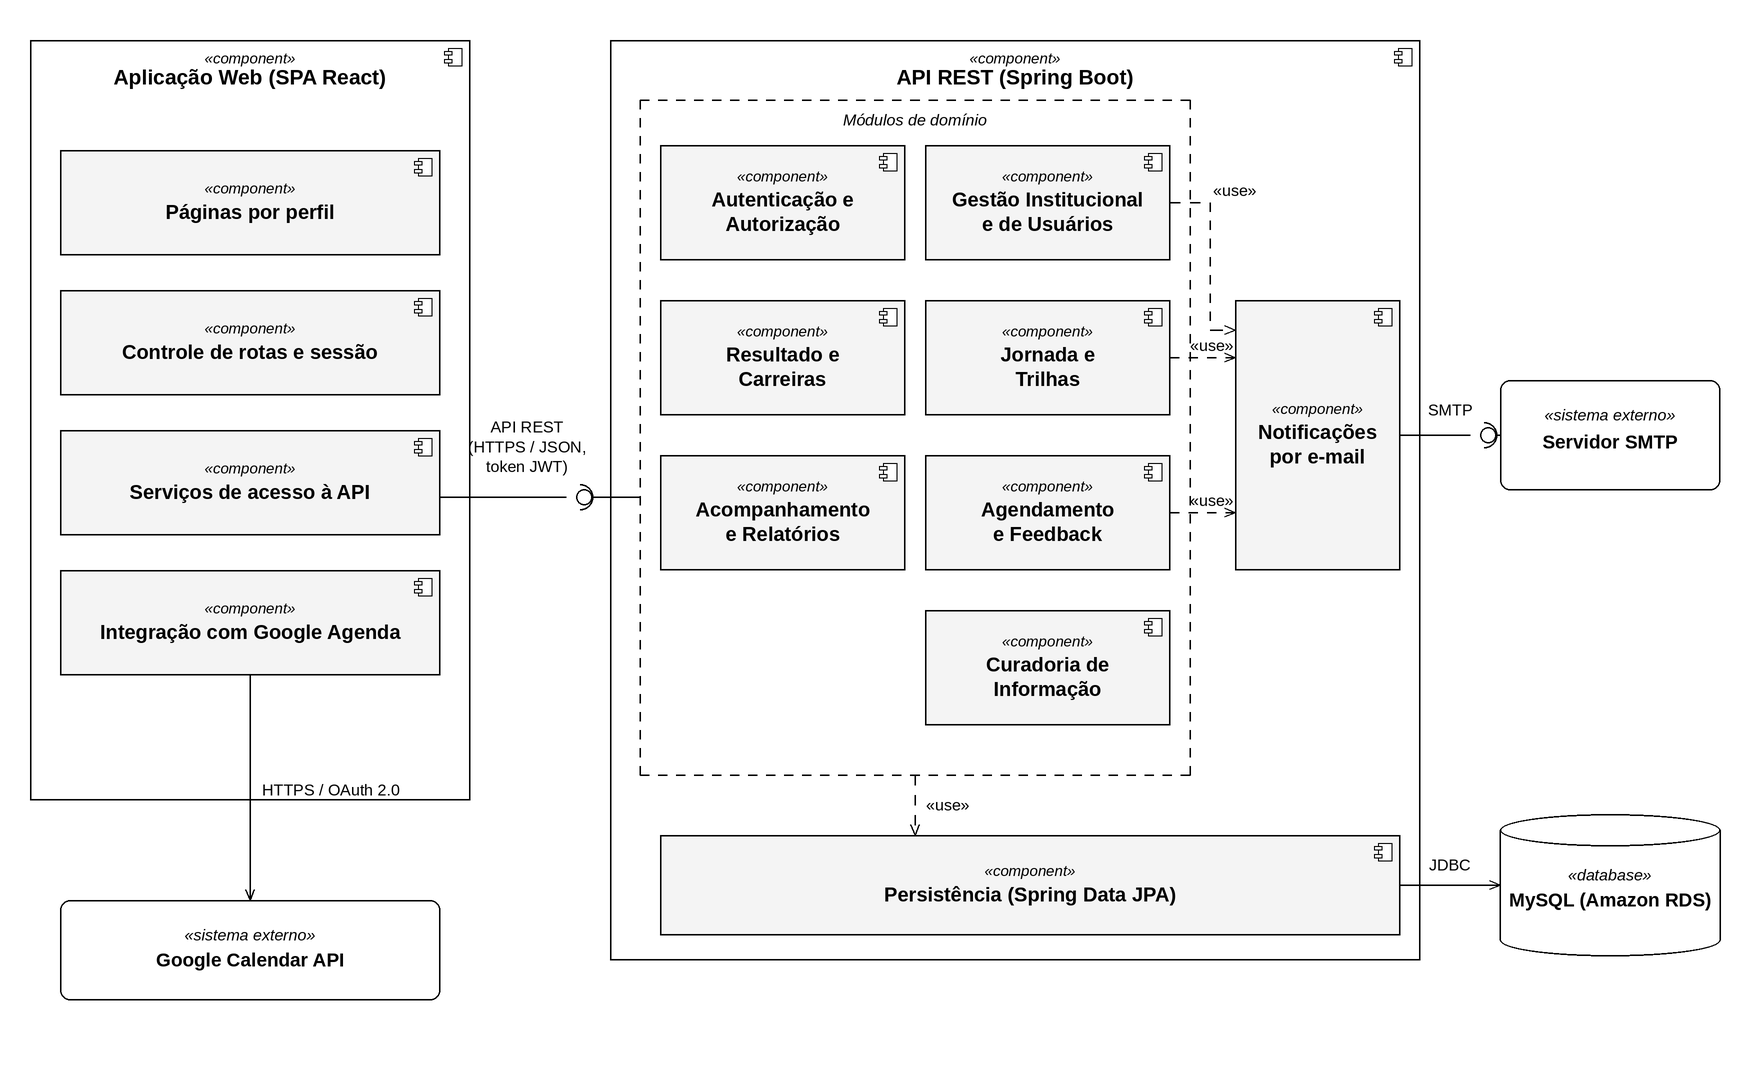
\includegraphics[width=\textwidth]{img/fig-cap4-componentes.png}
    \legend{Fonte: Autoria própria (2026).}
\end{figure}

A API REST agrupa seus módulos de domínio de acordo com os requisitos funcionais que atendem, todos apoiados no componente de persistência. O componente de notificações é utilizado pelos módulos que precisam enviar mensagens eletrônicas: o cadastro de usuários (primeiro acesso), a jornada (alerta de dúvida) e o \textit{feedback} ao aluno. A integração com o Google Calendar ocorre a partir da aplicação \textit{web}, com a autorização do próprio profissional de orientação, de modo que o servidor não armazena credenciais da conta Google.

Quanto à implantação, os arquivos estáticos da aplicação \textit{web}, gerados no processo de \textit{build}, são distribuídos pelo Amazon S3 e pela rede de distribuição de conteúdo Amazon CloudFront; o servidor de aplicação é executado em ambiente de nuvem da Amazon Web Services (AWS); e os dados são mantidos em uma instância gerenciada de MySQL no Amazon RDS \cite{aws2026}. A organização detalhada dos nós de execução corresponde à etapa de implementação.

\section{Projeto dos Componentes}

O projeto de componentes detalha a estrutura interna e as interfaces de cada componente definido na arquitetura, com o objetivo de obter módulos coesos, com baixo acoplamento entre si e interfaces bem definidas \cite{pressman2021}. No \textit{SyncCarreira}, cada módulo de domínio da API corresponde a um conjunto de controladores, serviços e repositórios e expõe um grupo de recursos REST. O \autoref{quadro-componentes} relaciona os componentes, os requisitos que atendem, suas principais classes e os recursos que expõem.

\begin{quadro}[H]
\ABNTEXfontereduzida
\caption{Componentes da API, requisitos atendidos e interfaces.}
\label{quadro-componentes}
\renewcommand{\arraystretch}{1.25}
\begin{tabularx}{\textwidth}{|>{\raggedright\arraybackslash}p{3.4cm}|>{\raggedright\arraybackslash}p{2.2cm}|>{\raggedright\arraybackslash}X|>{\raggedright\arraybackslash}p{4.5cm}|}
\hline
\textbf{Componente} & \textbf{Requisitos} & \textbf{Principais classes} & \textbf{Recursos REST} \\
\hline
Autenticação e Autorização & RNF-01 & AuthorizationServerConfig, ResourceServerConfig, AuthService, PasswordRecoverService & /oauth2/token, /auth/new-password, /users/me \\
\hline
Gestão Institucional e de Usuários & RF-01, RF-02 & InstitutionService, SchoolClassService, PsychologistService, StudentService, UserService & /institutions, /classes, /psychologists, /students, /users \\
\hline
Jornada e Trilhas & RF-10, RF-11, RF-13, RF-14, RF-15 & TrailService, QuestionService, AnswerService, SynthesisService, JourneyService, JourneyHistoryService, StudentProfileService & /trails, /questions, /answers, /syntheses, /journey/doubt, /journeys/me, /students/me \\
\hline
Resultado e Carreiras & RF-12 & JourneyResultService, AreaScoreCalculator & /journey/result, /journeys/me/\{id\}/result \\
\hline
Acompanhamento e Relatórios & RF-03, RF-04, RF-07 & PsychologistPanelService, PsychologistReportService, JourneyReportWriter & /psychologist-panel/\{id\}, /psychologist-panel/\{id\}/reports \\
\hline
Curadoria de Informação & RF-06 & InformationLinkService & /information-links \\
\hline
Agendamento e Feedback & RF-05, RF-08, RF-09, RF-16 & AppointmentService, FeedbackService & /appointments, /feedbacks \\
\hline
Notificações & RF-04, RF-09 & EmailService, EmailEventListener, modelos Thymeleaf & interna (SMTP) \\
\hline
Persistência & — & Repositórios Spring Data JPA e projeções de consulta & interna (JDBC) \\
\hline
\end{tabularx}
\legend{Fonte: Autoria própria (2026).}
\end{quadro}

Algumas decisões de projeto são transversais aos componentes:

\begin{itemize}
  \item \textbf{objetos de transferência por operação}: cada operação utiliza objetos de entrada e de saída próprios, o que evita a exposição de atributos sensíveis, como a senha, e permite validar os dados na fronteira da API por meio de anotações de validação declarativa;
  \item \textbf{verificação de acesso na camada de serviço}: além da restrição por perfil aplicada às rotas, os serviços verificam se o recurso solicitado pertence ao usuário autenticado ou à sua instituição, impedindo o acesso a dados de terceiros mesmo quando o identificador é conhecido;
  \item \textbf{tratamento centralizado de exceções}: um manipulador global converte as exceções de negócio em respostas HTTP padronizadas — 404 para recurso inexistente, 403 para acesso negado, 409 para conflito ou duplicidade e 422 para violação de regra de negócio ou dado inválido —, com mensagem descritiva e, quando aplicável, a lista de campos rejeitados;
  \item \textbf{notificações assíncronas após a confirmação da transação}: o envio de mensagens eletrônicas é disparado por eventos tratados somente depois da confirmação (\textit{commit}) da transação que os originou e executado de forma assíncrona, com novas tentativas em caso de falha temporária do servidor de e-mail; assim, a resposta ao usuário não depende da disponibilidade desse servidor;
  \item \textbf{cálculo do leque de possibilidades}: a pontuação de cada área do conhecimento é sempre recalculada a partir dos interesses declarados no perfil e dos pesos das opções respondidas, e comparada ao valor máximo possível de cada área, o que evita favorecer áreas com mais pontos distribuídos no banco de questões;
  \item \textbf{controle de concorrência}: as operações sujeitas a requisições simultâneas, como o registro de respostas e de sínteses, são protegidas por restrições de unicidade no banco de dados e por novas tentativas automáticas em caso de bloqueio, retornando conflito em vez de erro interno.
\end{itemize}

Na aplicação \textit{web}, os componentes organizam-se em páginas, agrupadas por perfil de acesso; serviços de acesso à API, que encapsulam as chamadas HTTP e o envio do \textit{token}; um contexto de autenticação, que mantém os dados do usuário autenticado; e guardas de rota, que restringem cada página aos perfis autorizados e direcionam o aluno ao preenchimento do perfil antes de liberar as trilhas. A integração com o Google Agenda é encapsulada em um serviço próprio, responsável pela autorização da conta e pela criação, atualização e cancelamento dos eventos.

\section{Modelo de Dados}

O projeto de um banco de dados percorre etapas sucessivas: o projeto conceitual, que descreve a estrutura de informação do domínio de forma independente de considerações de implementação, de eficiência de armazenamento ou do Sistema Gerenciador de Banco de Dados (SGBD) adotado; o projeto lógico, que traduz esse esquema para o modelo de dados do SGBD escolhido; e o projeto físico, que define estruturas de armazenamento e de acesso \cite{elmasri2011}. No \textit{SyncCarreira}, o modelo de dados é definido por classes persistentes mapeadas para tabelas relacionais por meio da especificação \textit{Jakarta Persistence} (JPA), e o banco de dados adotado é o MySQL \cite{mysql2026}.

As Figuras \ref{fig_classes_projeto_a} e \ref{fig_classes_projeto_b} apresentam o diagrama de classes de projeto, com os atributos, os tipos e as multiplicidades efetivamente adotados. Para manter a legibilidade, os atributos registrados por área do conhecimento — Humanas, Exatas, Biológicas e Artes — são representados de forma agrupada, como score«Área» e affinity«Área», e o diagrama foi dividido em duas partes.

\begin{figure}[H]
    \centering
    \caption{Diagrama de classes de projeto: usuários, instituições e jornada.}
    \label{fig_classes_projeto_a}
    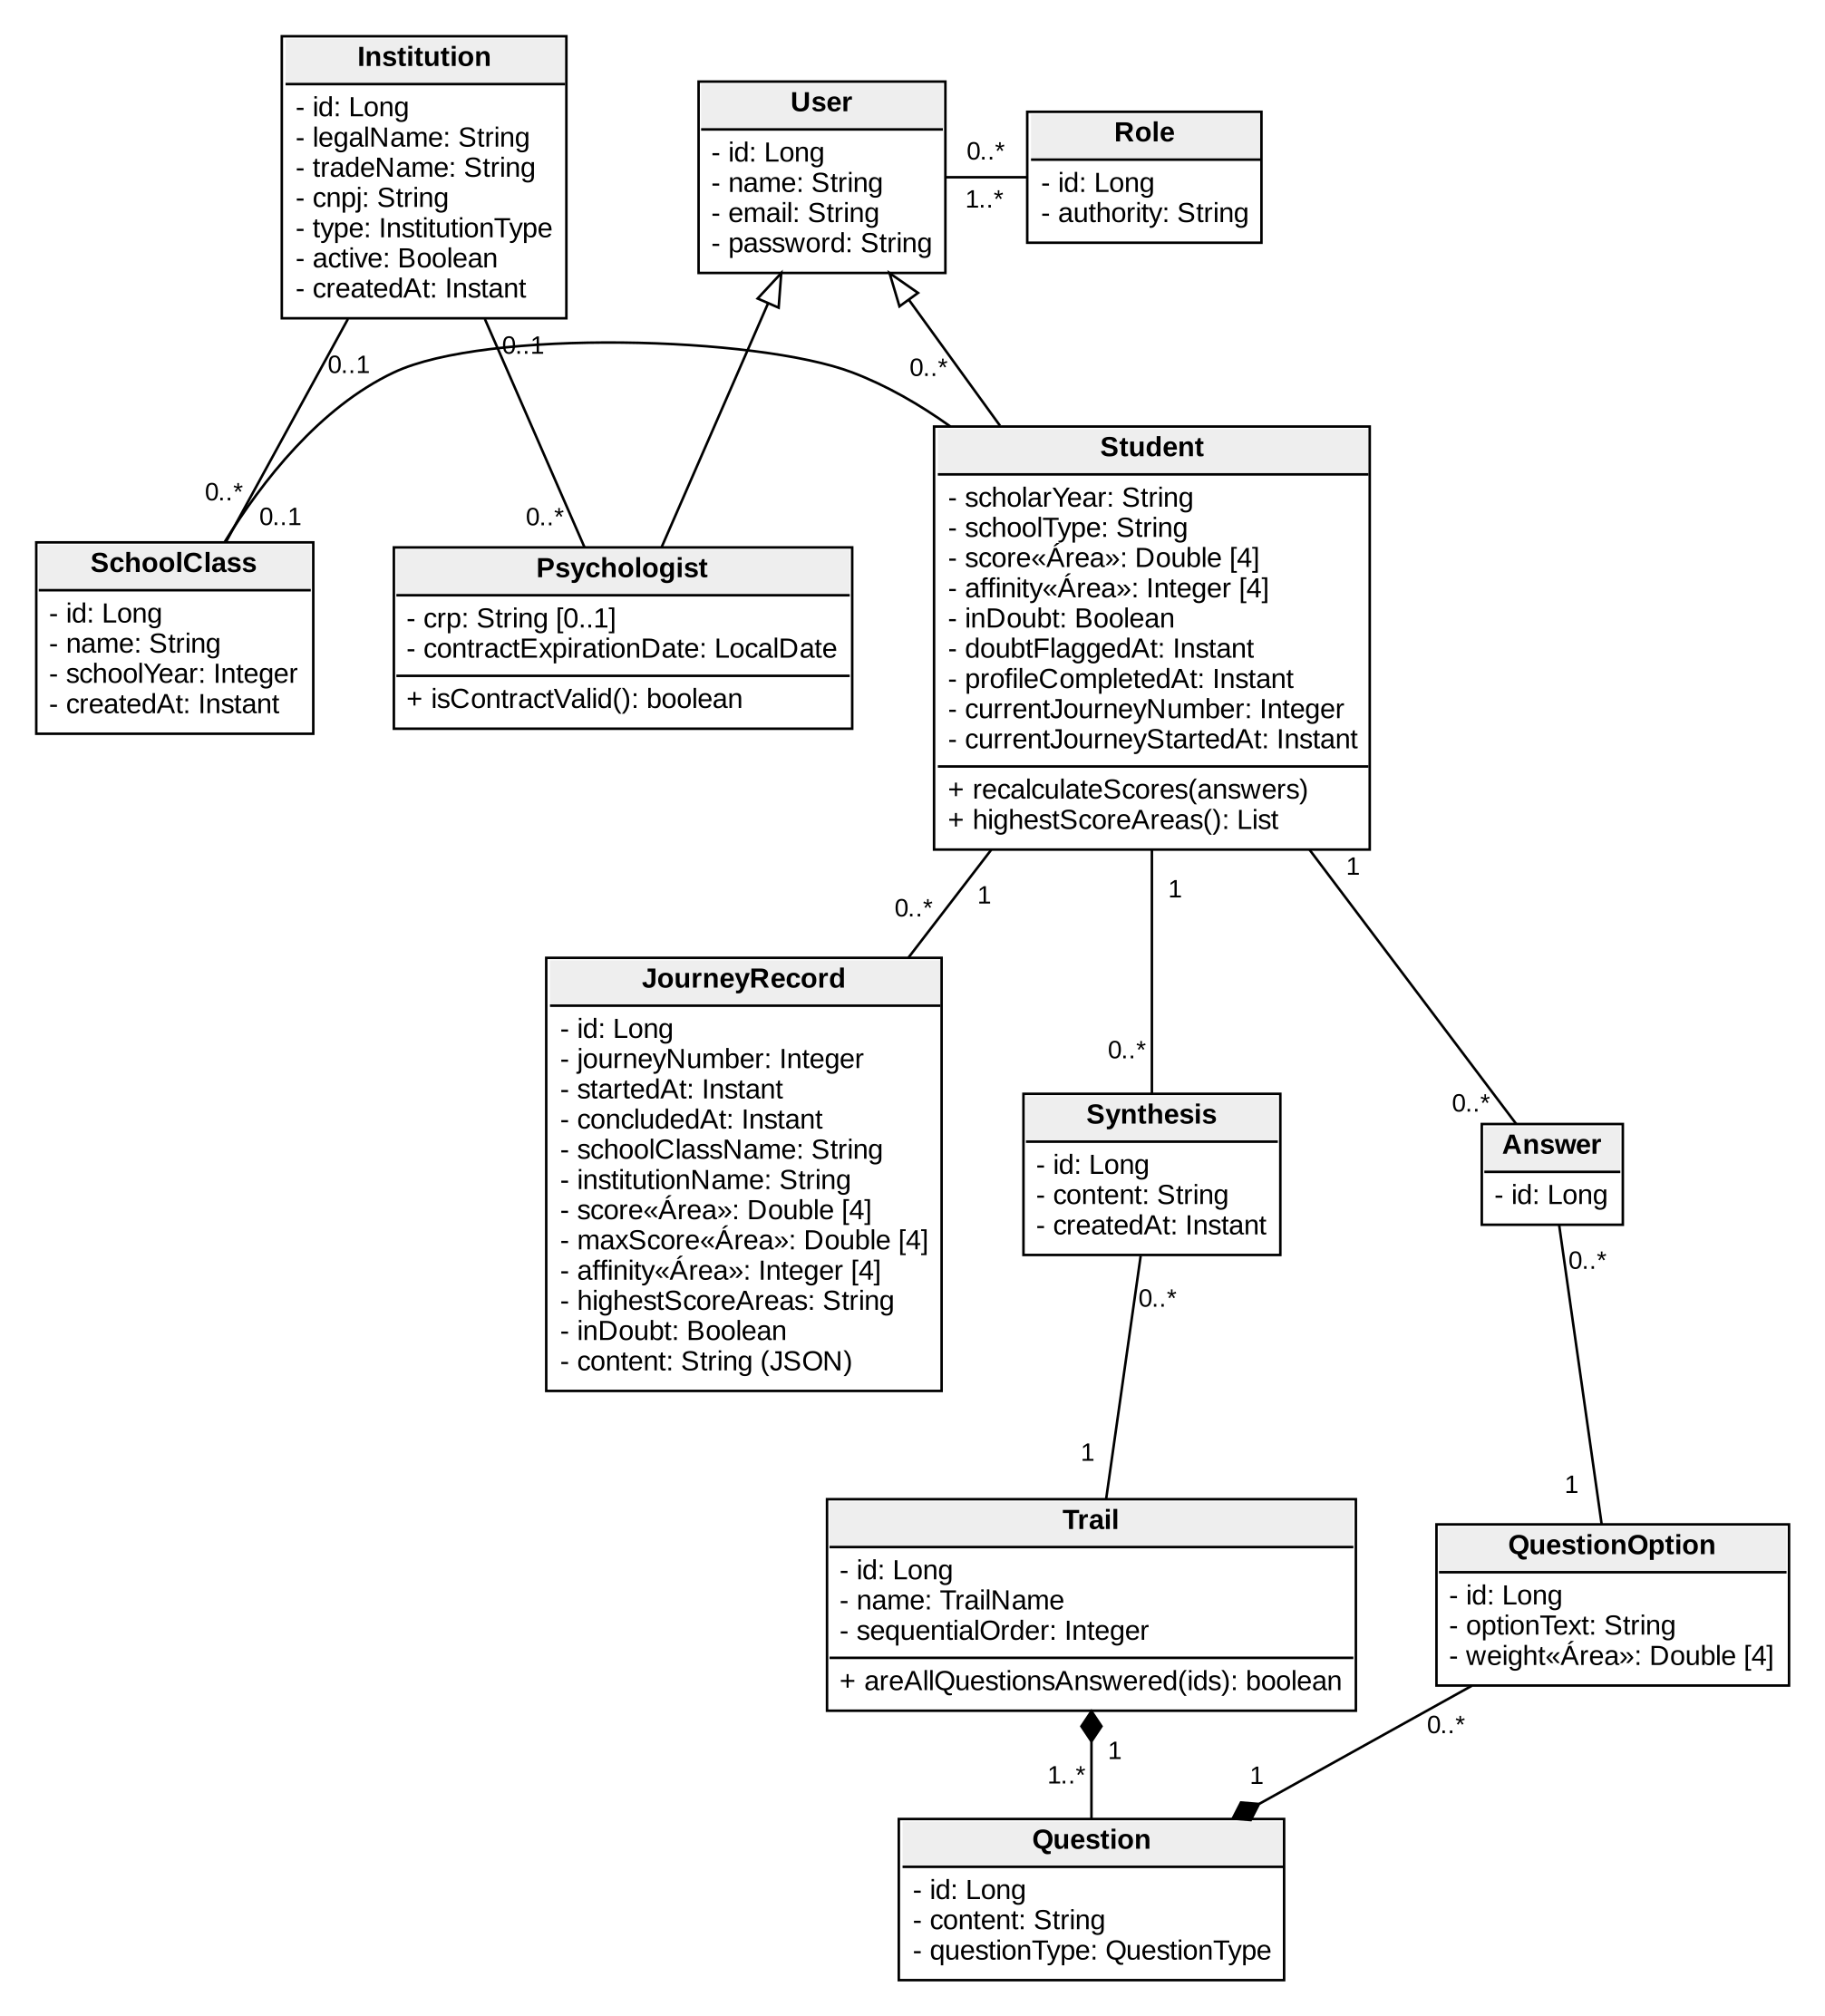
\includegraphics[width=0.92\textwidth]{img/fig-cap4-classes-projeto-a.png}
    \legend{Fonte: Autoria própria (2026).}
\end{figure}

\begin{figure}[H]
    \centering
    \caption{Diagrama de classes de projeto: acompanhamento, conteúdo e enumerações.}
    \label{fig_classes_projeto_b}
    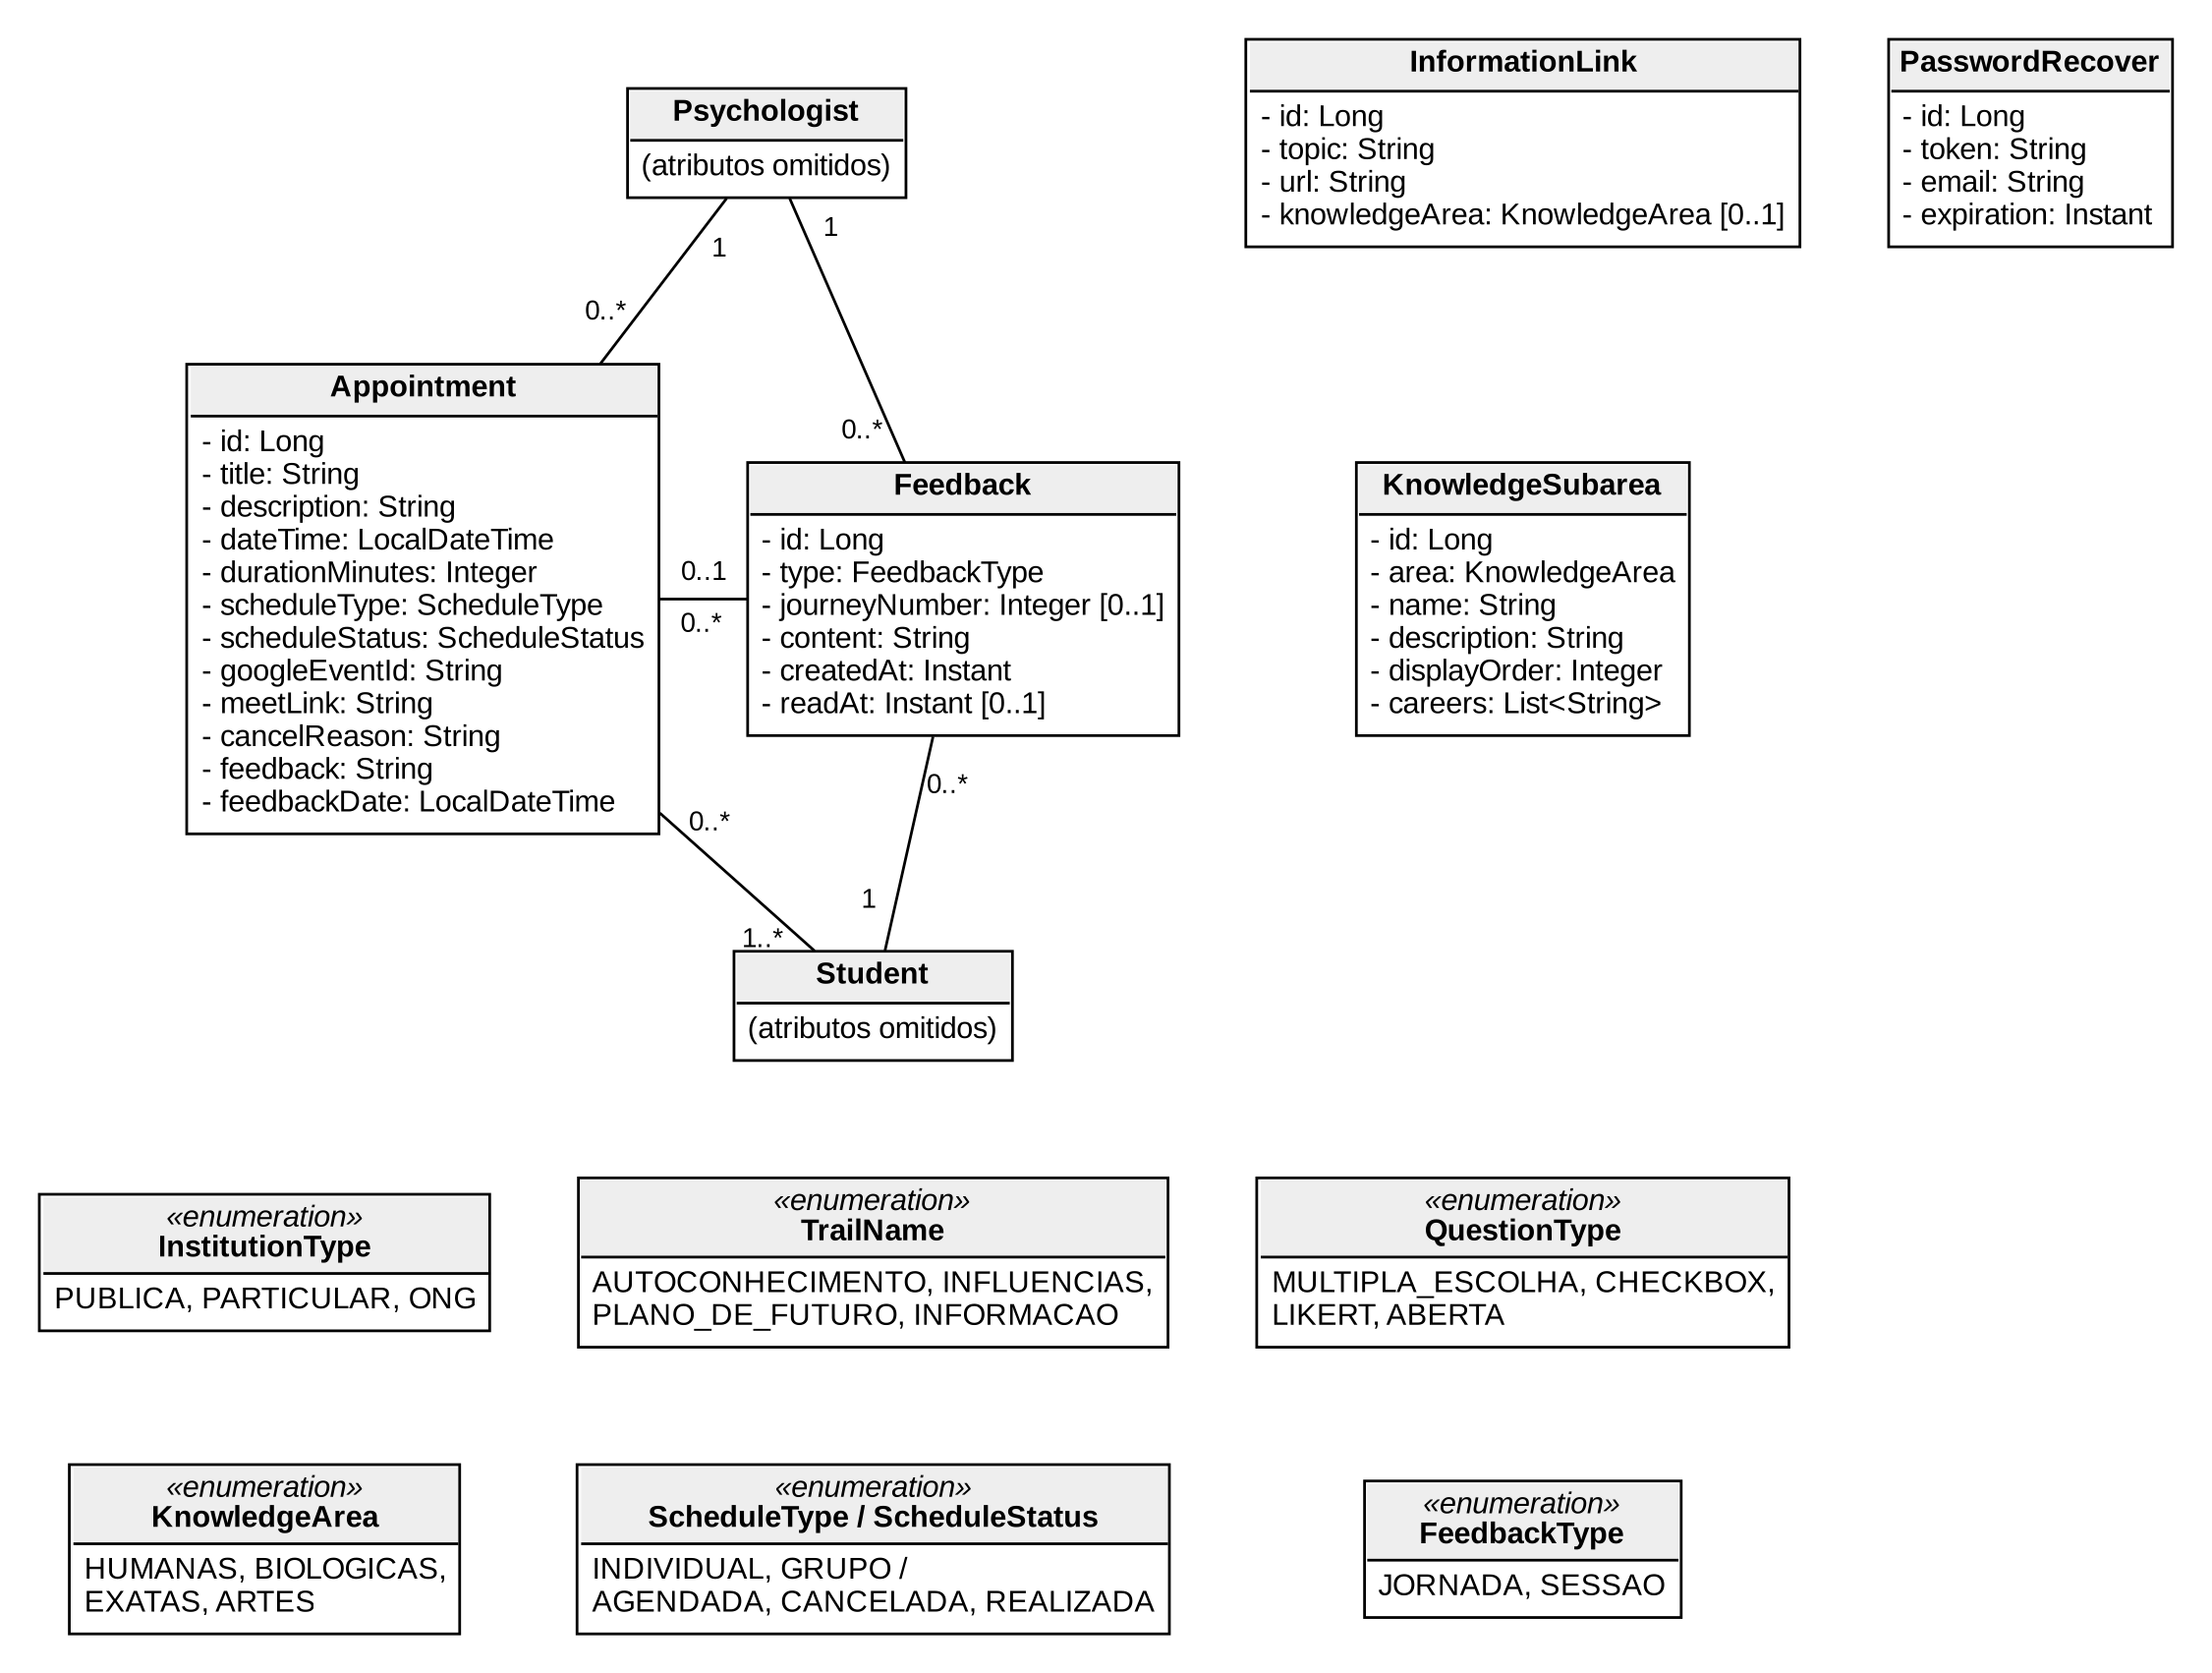
\includegraphics[width=0.98\textwidth]{img/fig-cap4-classes-projeto-b.png}
    \legend{Fonte: Autoria própria (2026).}
\end{figure}

O \autoref{quadro-tabelas} relaciona as classes persistentes às respectivas tabelas do banco de dados.

\begin{quadro}[H]
\ABNTEXfontereduzida
\caption{Classes persistentes e tabelas do banco de dados.}
\label{quadro-tabelas}
\renewcommand{\arraystretch}{1.25}
\begin{tabularx}{\textwidth}{|>{\raggedright\arraybackslash}p{3.9cm}|>{\raggedright\arraybackslash}p{4.9cm}|>{\raggedright\arraybackslash}X|}
\hline
\textbf{Classe} & \textbf{Tabela} & \textbf{Conteúdo} \\
\hline
User, Role & tb\_usuario, tb\_role, tb\_usuario\_role & Dados comuns de acesso e perfis de acesso de cada usuário. \\
\hline
Psychologist & tb\_psicologa & Dados específicos do profissional de orientação e vínculo com a instituição. \\
\hline
Student & tb\_aluno & Dados do aluno, interesses por área, pontuação da jornada em andamento e sinalização de dúvida. \\
\hline
Institution, SchoolClass & tb\_instituicao, tb\_turma & Instituições parceiras e suas turmas. \\
\hline
Trail, Question, QuestionOption & tb\_trilha, tb\_pergunta, tb\_opcao\_pergunta & Banco fixo de questões, com os pesos de cada opção por área. \\
\hline
Answer, Synthesis & tb\_respostas\_aluno, tb\_sintese & Respostas e sínteses da jornada em andamento. \\
\hline
JourneyRecord & tb\_jornada\_concluida & Registro imutável de cada jornada concluída. \\
\hline
KnowledgeSubarea & tb\_subarea\_conhecimento, tb\_subarea\_carreira & Subáreas do conhecimento e exemplos de carreiras do leque de possibilidades. \\
\hline
InformationLink & tb\_link\_informacao & Fontes externas curadas para a trilha de Informação. \\
\hline
Appointment & tb\_agendamento, tb\_agendamento\_aluno & Sessões de orientação e alunos convocados. \\
\hline
Feedback & tb\_feedback & Feedbacks individuais de jornada e de sessão. \\
\hline
PasswordRecover & tb\_senha\_recuperacao & Tokens temporários de definição de senha. \\
\hline
\end{tabularx}
\legend{Fonte: Autoria própria (2026).}
\end{quadro}

As principais decisões do modelo de dados são as seguintes:

\begin{itemize}
  \item \textbf{herança por tabelas associadas}: a classe User concentra os atributos comuns e é especializada em Psychologist e Student, cada uma com tabela própria ligada à tabela de usuários pela chave primária (estratégia \textit{joined}); essa estratégia evita colunas nulas que seriam necessárias em uma tabela única e preserva a integridade referencial. O Administrador não possui atributos próprios e é identificado apenas pelo perfil de acesso;
  \item \textbf{registro imutável das jornadas concluídas}: ao término de cada jornada, o sistema grava em JourneyRecord uma cópia das pontuações, dos valores máximos por área, dos interesses declarados e, em formato JSON, das questões, respostas, sínteses e \textit{links} daquela jornada. Essa desnormalização intencional garante que o histórico e o resultado de uma jornada concluída não se alterem quando o banco de questões, os pesos ou o perfil do aluno forem modificados, e permite reiniciar as trilhas em um novo ciclo;
  \item \textbf{restrições de unicidade}: o banco impede o registro de mais de uma síntese por aluno e trilha, de mais de um registro por número de jornada do aluno e de mais de um \textit{feedback} por aluno em uma mesma jornada ou sessão;
  \item \textbf{exclusão em cascata}: sínteses, jornadas concluídas e \textit{feedbacks} são removidos automaticamente com o aluno ou o profissional correspondente, em atendimento ao direito de eliminação de dados previsto na LGPD \cite{brasil2018lgpd};
  \item \textbf{enumerações persistidas como texto}: tipos de instituição, nomes de trilha, tipos de questão, áreas do conhecimento e situações de sessão são gravados por nome, o que torna os registros legíveis e independentes da ordem de declaração;
  \item \textbf{carga inicial}: os perfis de acesso, as trilhas, o banco de questões — trinta questões e 138 opções de resposta com pesos por área — e as vinte subáreas do conhecimento são carregados por \textit{script} de inicialização no ambiente de testes.
\end{itemize}

\section{Projeto da Interface do Usuário}

O projeto da interface do usuário define a organização das telas, a navegação entre elas e os padrões visuais e de interação adotados. Para orientar essas decisões, foram consideradas as heurísticas de usabilidade de \citeonline{nielsen2024}, em especial a visibilidade do estado do sistema, a correspondência entre o sistema e o mundo real, a prevenção de erros e o reconhecimento em lugar da memorização.

A interface organiza-se por perfil de acesso. Após a autenticação, cada usuário é direcionado à sua tela inicial e dispõe de um menu de navegação com as opções permitidas ao seu perfil: o profissional de orientação acessa o painel de progresso, os agendamentos e a curadoria de \textit{links}; o aluno acessa as trilhas, o panorama da jornada, o perfil e os agendamentos; e o Administrador acessa a gestão de usuários, turmas e instituições. A \autoref{fig_navegacao} apresenta o mapa de navegação da aplicação, com as telas e os respectivos endereços.

\begin{figure}[H]
    \centering
    \caption{Mapa de navegação da interface do SyncCarreira.}
    \label{fig_navegacao}
    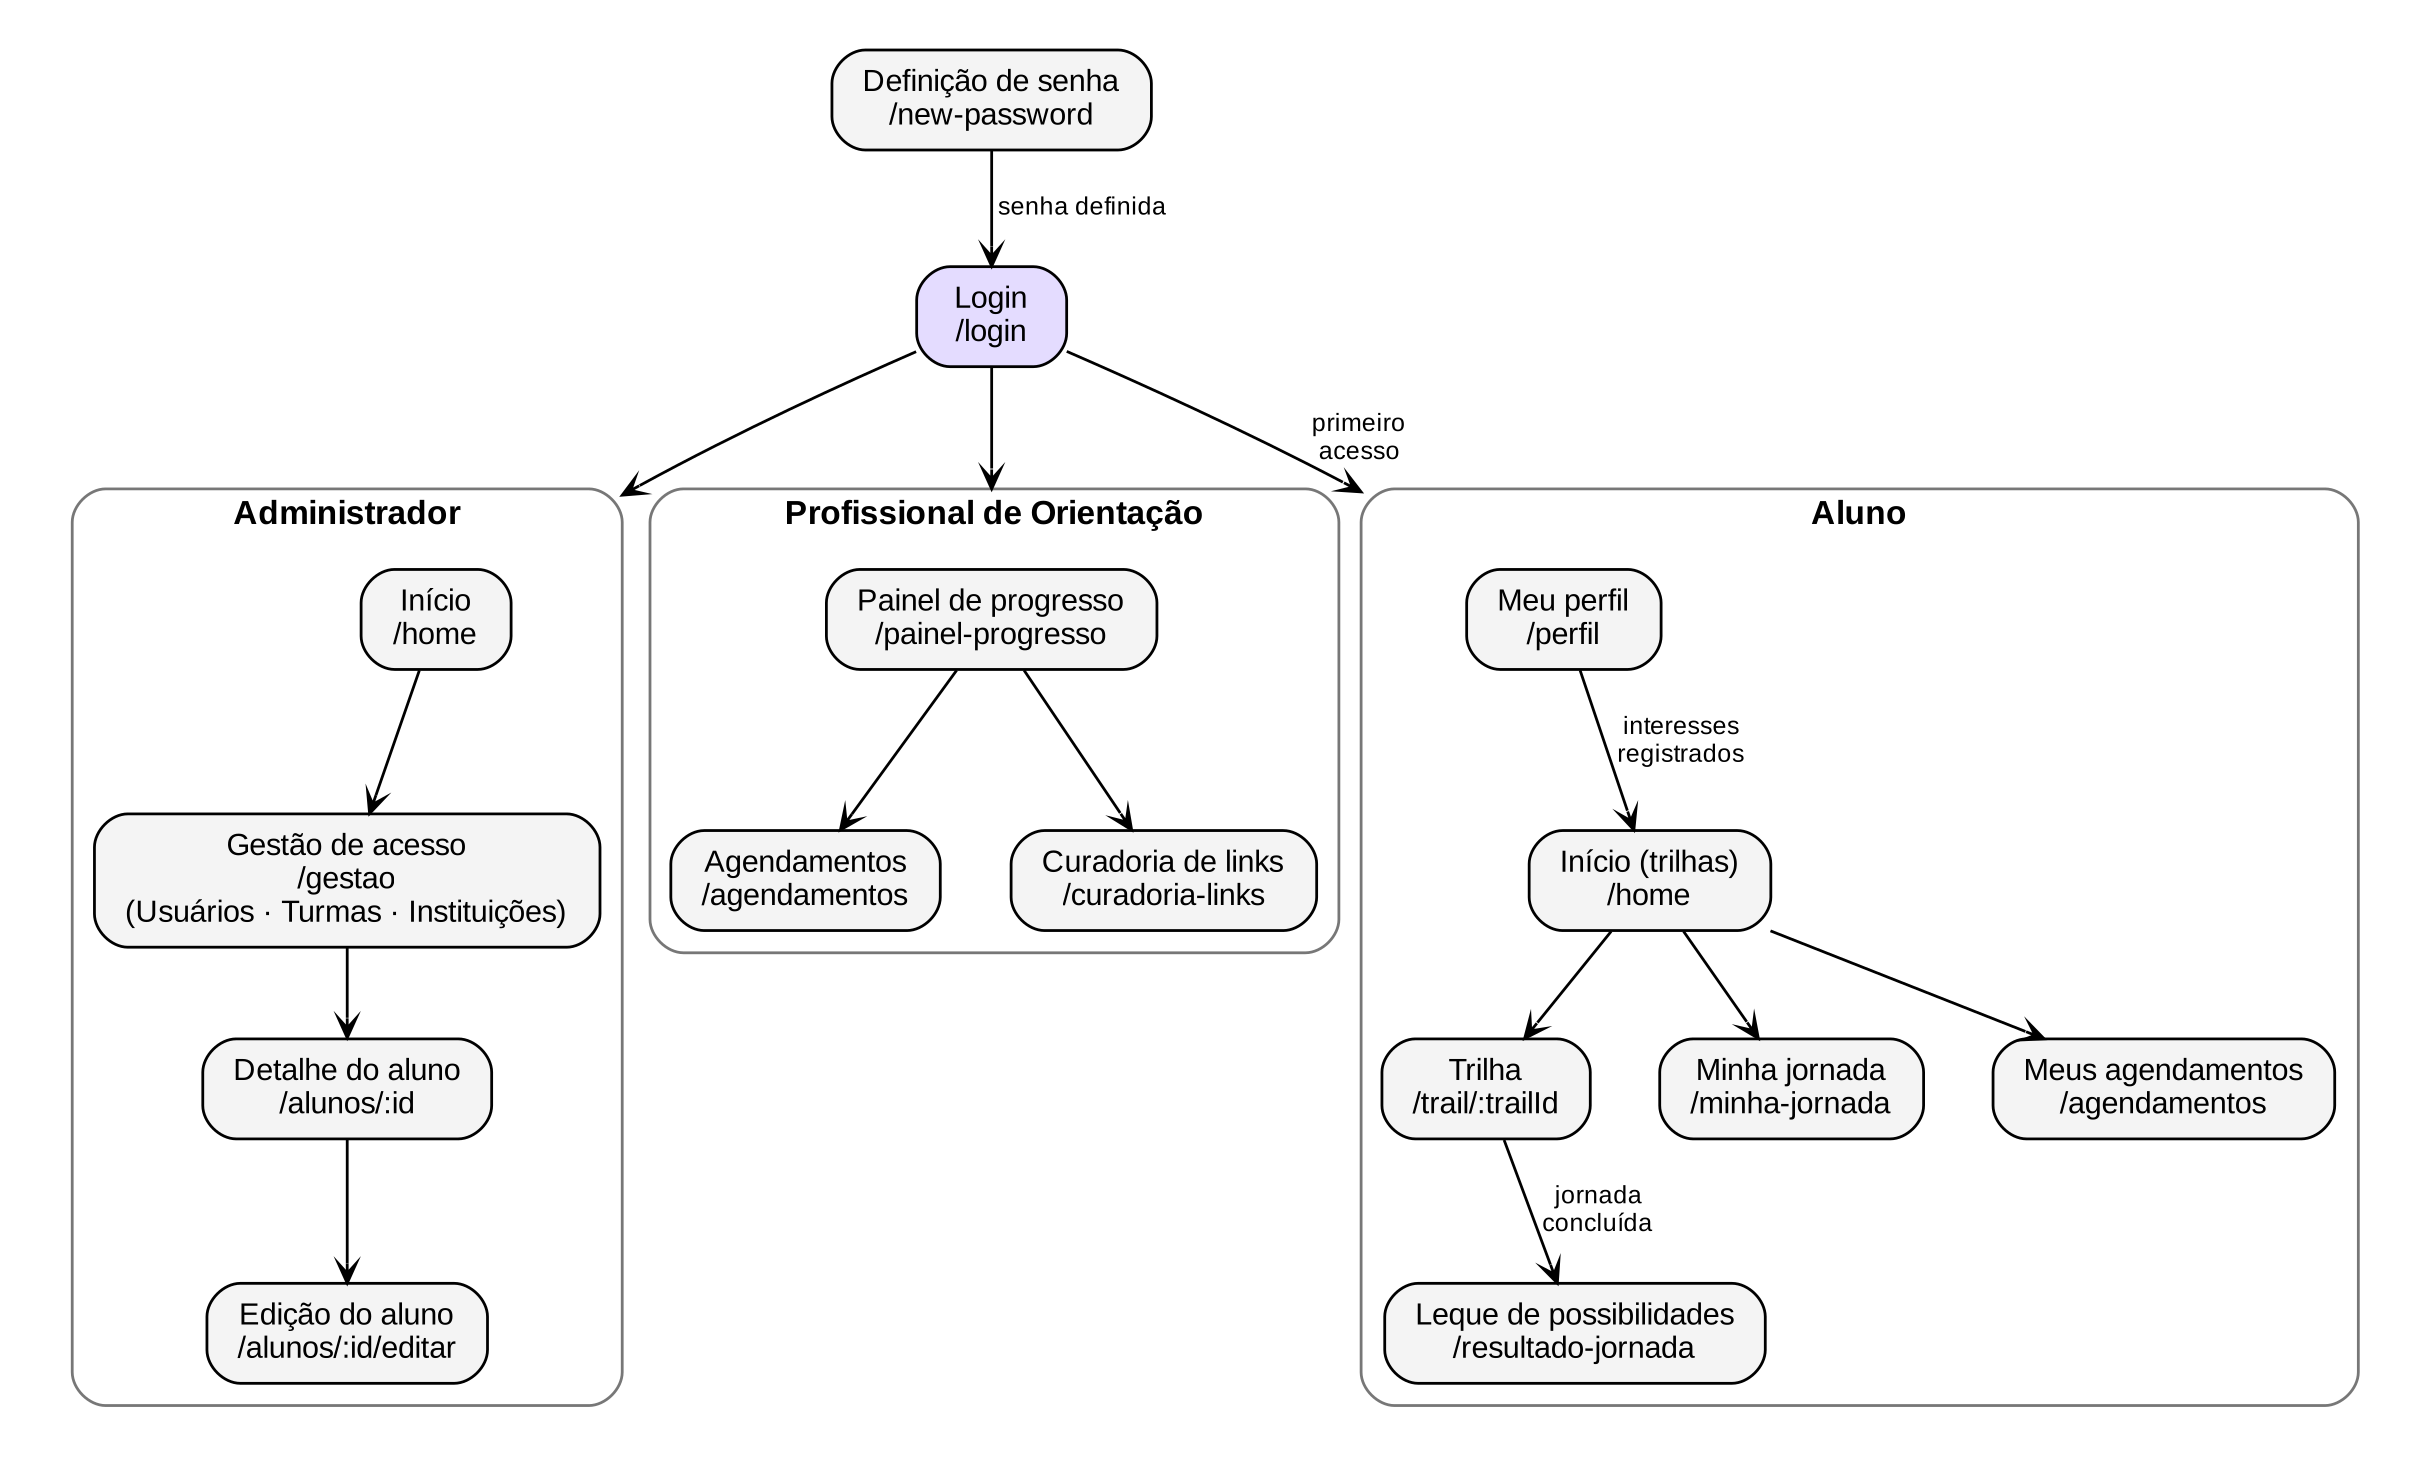
\includegraphics[width=\textwidth]{img/fig-cap4-navegacao.png}
    \legend{Fonte: Autoria própria (2026).}
\end{figure}

Os principais padrões adotados na interface são os seguintes:

\begin{itemize}
  \item \textbf{visibilidade do estado do sistema}: as trilhas exibem sua situação (bloqueada, disponível, em andamento ou concluída) e o percentual de progresso; as operações apresentam estados de carregamento, confirmação e erro, com opção de nova tentativa;
  \item \textbf{prevenção de erros}: trilhas bloqueadas não podem ser abertas, o campo de síntese só é exibido após a resposta de todas as questões e ações irreversíveis, como a exclusão de uma conta, exigem confirmação;
  \item \textbf{linguagem do domínio}: os rótulos utilizam os termos do processo de orientação — trilha, síntese, leque de possibilidades, sessão — e o resultado da jornada é acompanhado de aviso explícito de que não constitui diagnóstico;
  \item \textbf{identidade visual centralizada}: cores, tipografia, raios de borda e sombras são definidos em um único conjunto de variáveis de estilo, com cor primária violeta e fundo neutro, assegurando consistência entre as telas;
  \item \textbf{responsividade e acessibilidade}: as telas adaptam sua disposição a larguras menores por meio de pontos de quebra, e os componentes interativos utilizam atributos de acessibilidade para leitores de tela, como rótulos, estados expandidos e regiões de atualização dinâmica.
\end{itemize}

As Figuras \ref{fig_tela_login} a \ref{fig_tela_leque} apresentam as principais telas do sistema.

% TODO: substituir o quadro cinza pela captura de tela (\includegraphics[width=0.85\textwidth]{img/...})
\begin{figure}[H]
    \centering
    \caption{Tela de autenticação.}
    \label{fig_tela_login}
    \fcolorbox{gray}{gray!8}{\parbox[c][4.5cm][c]{0.7\textwidth}{\centering\textit{[Inserir captura de tela]}}}
    \legend{Fonte: Autoria própria (2026).}
\end{figure}

% TODO: substituir o quadro cinza pela captura de tela (\includegraphics[width=0.85\textwidth]{img/...})
\begin{figure}[H]
    \centering
    \caption{Painel de progresso do profissional de orientação.}
    \label{fig_tela_painel}
    \fcolorbox{gray}{gray!8}{\parbox[c][4.5cm][c]{0.7\textwidth}{\centering\textit{[Inserir captura de tela]}}}
    \legend{Fonte: Autoria própria (2026).}
\end{figure}

% TODO: substituir o quadro cinza pela captura de tela (\includegraphics[width=0.85\textwidth]{img/...})
\begin{figure}[H]
    \centering
    \caption{Tela de trilha com o registro da síntese.}
    \label{fig_tela_trilha}
    \fcolorbox{gray}{gray!8}{\parbox[c][4.5cm][c]{0.7\textwidth}{\centering\textit{[Inserir captura de tela]}}}
    \legend{Fonte: Autoria própria (2026).}
\end{figure}

% TODO: substituir o quadro cinza pela captura de tela (\includegraphics[width=0.85\textwidth]{img/...})
\begin{figure}[H]
    \centering
    \caption{Tela do leque de possibilidades de carreira.}
    \label{fig_tela_leque}
    \fcolorbox{gray}{gray!8}{\parbox[c][4.5cm][c]{0.7\textwidth}{\centering\textit{[Inserir captura de tela]}}}
    \legend{Fonte: Autoria própria (2026).}
\end{figure}

\section{Diagramas de Interação}

Os diagramas de sequência representam a colaboração entre os objetos que realizam um comportamento, evidenciando a ordem temporal das mensagens trocadas entre eles \cite{omg2017uml}. Foram modelados os três fluxos de maior complexidade do sistema, por envolverem regras de negócio encadeadas, processamento assíncrono ou integração com sistema externo.

A \autoref{fig_seq_sintese} apresenta o registro da síntese de uma trilha. A API verifica se a trilha está liberada para o aluno e se todas as suas questões foram respondidas antes de registrar a síntese; em seguida, caso todas as trilhas estejam concluídas, registra a jornada no histórico do aluno. As violações dessas condições resultam em respostas de acesso negado (403), regra de negócio violada (422) ou síntese já registrada (409).

\begin{figure}[H]
    \centering
    \caption{Diagrama de sequência do registro de síntese da trilha.}
    \label{fig_seq_sintese}
    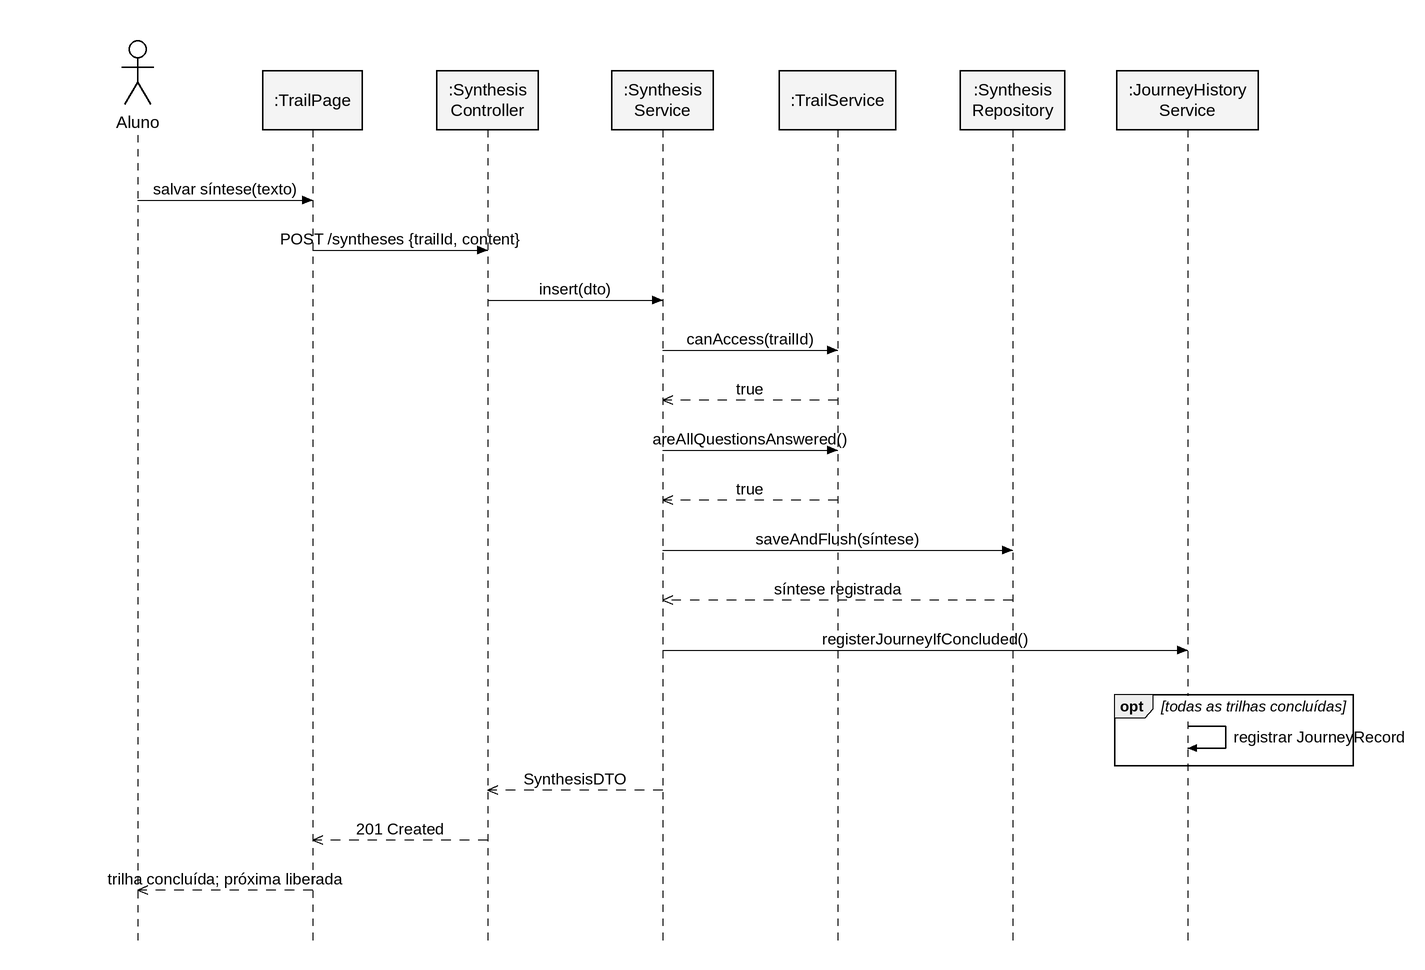
\includegraphics[width=\textwidth]{img/fig-cap4-seq-sintese.png}
    \legend{Fonte: Autoria própria (2026).}
\end{figure}

A \autoref{fig_seq_duvida} apresenta a sinalização de dúvida pelo aluno ao final da jornada. A resposta ao aluno é devolvida assim que a sinalização é gravada; a mensagem eletrônica destinada a cada profissional de orientação com contrato vigente na instituição é enviada somente após a confirmação da transação e de forma assíncrona, de modo que eventual indisponibilidade do servidor de e-mail não impede o registro da sinalização.

\begin{figure}[H]
    \centering
    \caption{Diagrama de sequência da sinalização de dúvida.}
    \label{fig_seq_duvida}
    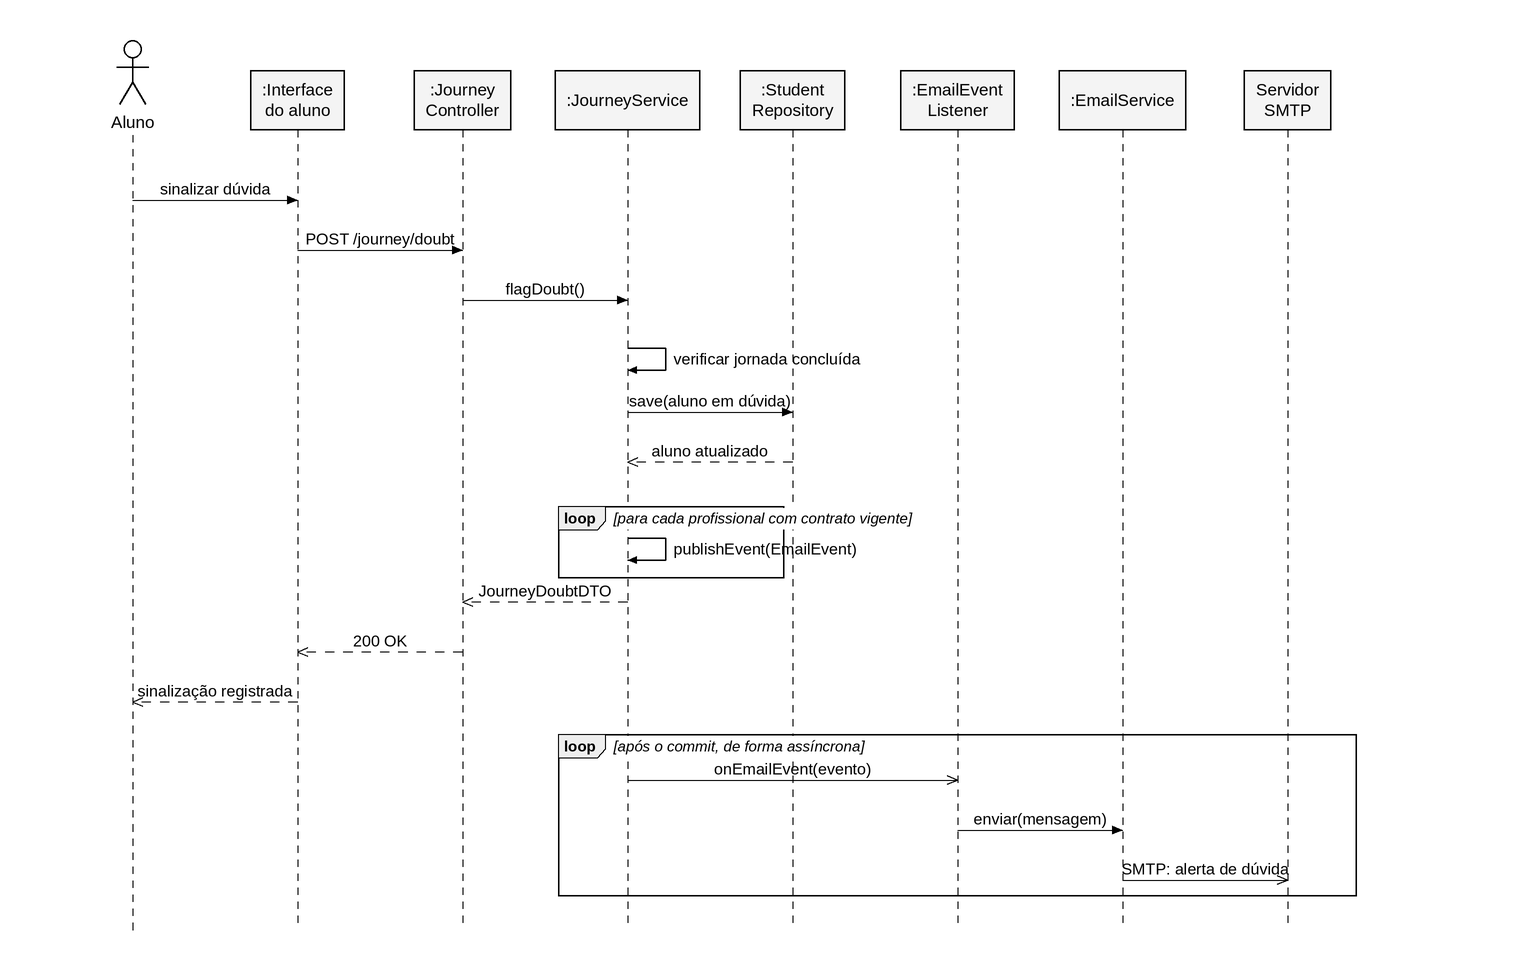
\includegraphics[width=\textwidth]{img/fig-cap4-seq-duvida.png}
    \legend{Fonte: Autoria própria (2026).}
\end{figure}

A \autoref{fig_seq_agendamento} apresenta o agendamento de uma sessão de orientação. Quando a conta do Google Agenda está conectada, a aplicação \textit{web} cria primeiro o evento, com os alunos como convidados e o \textit{link} de videoconferência, e depois registra a sessão na API. Se a API rejeitar o registro — por exemplo, por envolver aluno de outra instituição —, a aplicação cancela o evento recém-criado, evitando convites para uma sessão inexistente.

\begin{figure}[H]
    \centering
    \caption{Diagrama de sequência do agendamento de sessão.}
    \label{fig_seq_agendamento}
    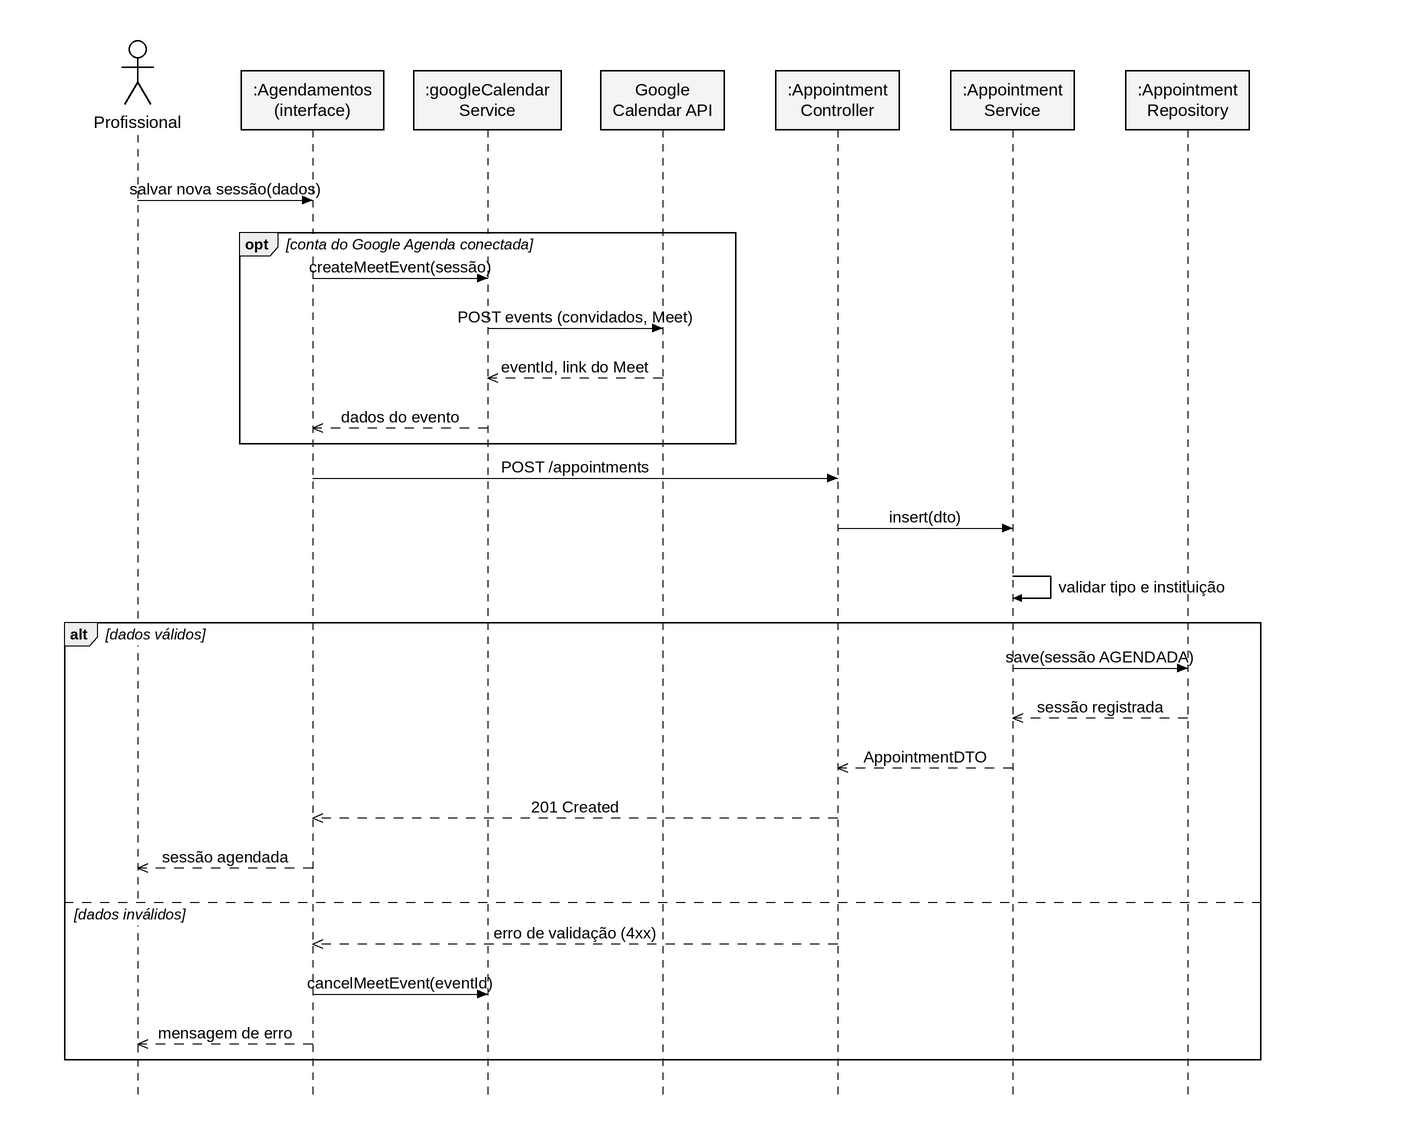
\includegraphics[width=\textwidth]{img/fig-cap4-seq-agendamento.png}
    \legend{Fonte: Autoria própria (2026).}
\end{figure}

\section{Tecnologias Utilizadas}

A seleção das tecnologias considerou a maturidade e a documentação de cada ferramenta, sua adequação aos requisitos não funcionais e o domínio prévio da equipe. O servidor foi desenvolvido em Java com o ecossistema Spring, que oferece módulos integrados para a construção de APIs, persistência, segurança e documentação \cite{spring2026}. A aplicação \textit{web} utiliza a biblioteca React, baseada em componentes reutilizáveis e na atualização declarativa da interface \cite{react2026}. O \autoref{quadro-tecnologias} apresenta as tecnologias adotadas e sua função no projeto.

\begin{quadro}[H]
\ABNTEXfontereduzida
\caption{Tecnologias utilizadas no SyncCarreira.}
\label{quadro-tecnologias}
\renewcommand{\arraystretch}{1.25}
\begin{tabularx}{\textwidth}{|>{\raggedright\arraybackslash}p{2.8cm}|>{\raggedright\arraybackslash}p{4.9cm}|>{\raggedright\arraybackslash}p{1.8cm}|>{\raggedright\arraybackslash}X|}
\hline
\textbf{Camada} & \textbf{Tecnologia} & \textbf{Versão} & \textbf{Função no projeto} \\
\hline
Servidor & Java & 21 & Linguagem do servidor. \\
\hline
Servidor & Spring Boot & 4.0.5 & Base da aplicação, configuração e servidor HTTP embarcado. \\
\hline
Servidor & Spring Security, Authorization Server e Resource Server & —\textsuperscript{1} & Autenticação, emissão e validação de \textit{tokens} JWT e autorização por perfil. \\
\hline
Servidor & Spring Data JPA e Hibernate & —\textsuperscript{1} & Mapeamento objeto-relacional e acesso aos dados. \\
\hline
Servidor & Jakarta Bean Validation & —\textsuperscript{1} & Validação declarativa dos dados de entrada. \\
\hline
Servidor & Spring Mail e Thymeleaf & —\textsuperscript{1} & Envio de mensagens eletrônicas a partir de modelos HTML. \\
\hline
Servidor & Spring Retry & 2.0.13 & Novas tentativas em falhas temporárias de e-mail e de bloqueio no banco. \\
\hline
Servidor & springdoc-openapi (Swagger UI) & 3.0.2 & Documentação automática da API (RNF-07). \\
\hline
Servidor & Apache POI & 5.4.1 & Geração dos relatórios em planilha (.xlsx). \\
\hline
Servidor & OpenPDF & 2.0.3 & Geração do registro da jornada em PDF. \\
\hline
Servidor & Lombok & —\textsuperscript{1} & Geração de métodos de acesso e construtores. \\
\hline
Servidor & Gradle & 9.4.1 & Automação de \textit{build} e gestão de dependências. \\
\hline
Dados & MySQL (Amazon RDS) & — & Banco de dados relacional dos ambientes de desenvolvimento e produção. \\
\hline
Dados & H2 Database & —\textsuperscript{1} & Banco em memória do ambiente de testes. \\
\hline
Aplicação \textit{web} & React & 18 & Construção da interface por componentes. \\
\hline
Aplicação \textit{web} & React Router & 6 & Navegação entre telas e guardas de rota. \\
\hline
Aplicação \textit{web} & Axios & 1 & Cliente HTTP de acesso à API. \\
\hline
Aplicação \textit{web} & Vite & 5 & Servidor de desenvolvimento e \textit{build} da aplicação. \\
\hline
Integração & Google Identity Services e Google Calendar API & v3 & Autorização da conta Google e criação de eventos com videoconferência. \\
\hline
Infraestrutura & Amazon S3 e Amazon CloudFront & — & Hospedagem e distribuição dos arquivos estáticos da aplicação \textit{web}. \\
\hline
Qualidade & GitHub Actions, SonarCloud e JaCoCo & — & Compilação automática, análise estática e cobertura de testes a cada integração. \\
\hline
\end{tabularx}
{\footnotesize \textsuperscript{1} Versão gerenciada pelo Spring Boot 4.0.5.\par}
\legend{Fonte: Autoria própria (2026).}
\end{quadro}

\section{Segurança e Controle de Acesso}

Por tratar dados de orientação vocacional de estudantes, em sua maioria menores de idade, o \textit{SyncCarreira} está sujeito às exigências da Lei Geral de Proteção de Dados Pessoais quanto ao tratamento de dados de crianças e adolescentes \cite{brasil2018lgpd}. Além disso, a falha no controle de acesso ocupa a primeira posição entre os riscos de segurança mais críticos de aplicações \textit{web} \cite{owasp2021}. As decisões descritas a seguir respondem a esses dois condicionantes.

\subsection{Autenticação}

A autenticação baseia-se no protocolo OAuth 2.0, que define a emissão de \textit{tokens} de acesso por um servidor de autorização e seu uso pelo cliente nas requisições aos recursos protegidos \cite{hardt2012rfc6749}. O servidor de autorização integrado à API recebe o e-mail e a senha do usuário, valida as credenciais e emite um \textit{token} no formato JSON Web Token (JWT): uma estrutura autocontida e assinada digitalmente, que transporta as declarações sobre o usuário e cuja integridade pode ser verificada sem consulta ao banco de dados \cite{jones2015rfc7519}. O \textit{token} do \textit{SyncCarreira} contém o identificador do usuário e seus perfis de acesso, é assinado com chave RSA e tem validade de cinco horas. A aplicação \textit{web} armazena o \textit{token} e o envia no cabeçalho de autorização de cada requisição; ao receber uma resposta de não autenticado, descarta-o e direciona o usuário à tela de autenticação.

As senhas não são armazenadas em texto claro: são transformadas por meio da função de \textit{hash} BCrypt, projetada para ser computacionalmente custosa e incorporar um valor aleatório (\textit{salt}) a cada senha, o que dificulta ataques de dicionário e de força bruta \cite{provos1999}. As contas são criadas exclusivamente pelo Administrador; o próprio usuário define sua senha, com no mínimo oito caracteres, por meio de um \textit{link} de uso temporário enviado ao e-mail cadastrado. Na falha de autenticação, a mensagem devolvida é genérica, sem indicar se o erro está no e-mail ou na senha.

\subsection{Autorização}

O controle de acesso é aplicado em dois níveis. No primeiro, baseado em perfis, cada grupo de recursos da API é associado aos perfis autorizados — Administrador, Profissional de Orientação e Aluno —, e as requisições de perfis não autorizados são rejeitadas antes de alcançar a lógica de negócio. O \autoref{quadro-autorizacao} apresenta a matriz de autorização por perfil.

\begin{quadro}[H]
\ABNTEXfontereduzida
\caption{Matriz de autorização por perfil.}
\label{quadro-autorizacao}
\renewcommand{\arraystretch}{1.25}
\begin{tabularx}{\textwidth}{|>{\raggedright\arraybackslash}X|>{\raggedright\arraybackslash}p{2.8cm}|>{\raggedright\arraybackslash}p{2.8cm}|>{\raggedright\arraybackslash}p{2.7cm}|}
\hline
\textbf{Recurso} & \textbf{Administrador} & \textbf{Profissional} & \textbf{Aluno} \\
\hline
Usuários, instituições, turmas e profissionais & Gerencia & — & — \\
\hline
Alunos (cadastro, edição e exclusão) & Gerencia & Consulta & — \\
\hline
Banco de questões & Gerencia & Consulta & Consulta \\
\hline
Perfil, respostas, sínteses, jornada, histórico e resultado & — & — & Próprios dados \\
\hline
Painel de progresso e relatórios & Consulta & Própria instituição & — \\
\hline
Links de informação & Gerencia & Gerencia & Consulta na trilha \\
\hline
Sessões de orientação & Gerencia & Própria agenda & Consulta das próprias \\
\hline
Feedbacks & Consulta do status & Envia e exclui & Consulta e marca como lido \\
\hline
\end{tabularx}
\legend{Fonte: Autoria própria (2026).}
\end{quadro}

No segundo nível, os serviços verificam a propriedade e o escopo institucional de cada recurso. O aluno acessa apenas os próprios dados, identificados a partir do \textit{token}, e não a partir de parâmetros informados na requisição; o profissional de orientação acessa apenas o próprio painel e a própria agenda, e somente pode convocar para sessões alunos vinculados a turmas da sua instituição. Essa verificação impede que a simples alteração de um identificador na requisição dê acesso a dados de outro usuário ou de outra instituição, em atendimento aos requisitos RNF-01 e RNF-08.

O acesso às trilhas também é controlado pelo sistema, conforme a regra de negócio RN-01. A \autoref{fig_estados_acesso} apresenta o ciclo de vida do acesso de um usuário, e a \autoref{fig_estados_trilha}, os estados de uma trilha na jornada do aluno.

\begin{figure}[H]
    \centering
    \caption{Diagrama de estados do acesso do usuário.}
    \label{fig_estados_acesso}
    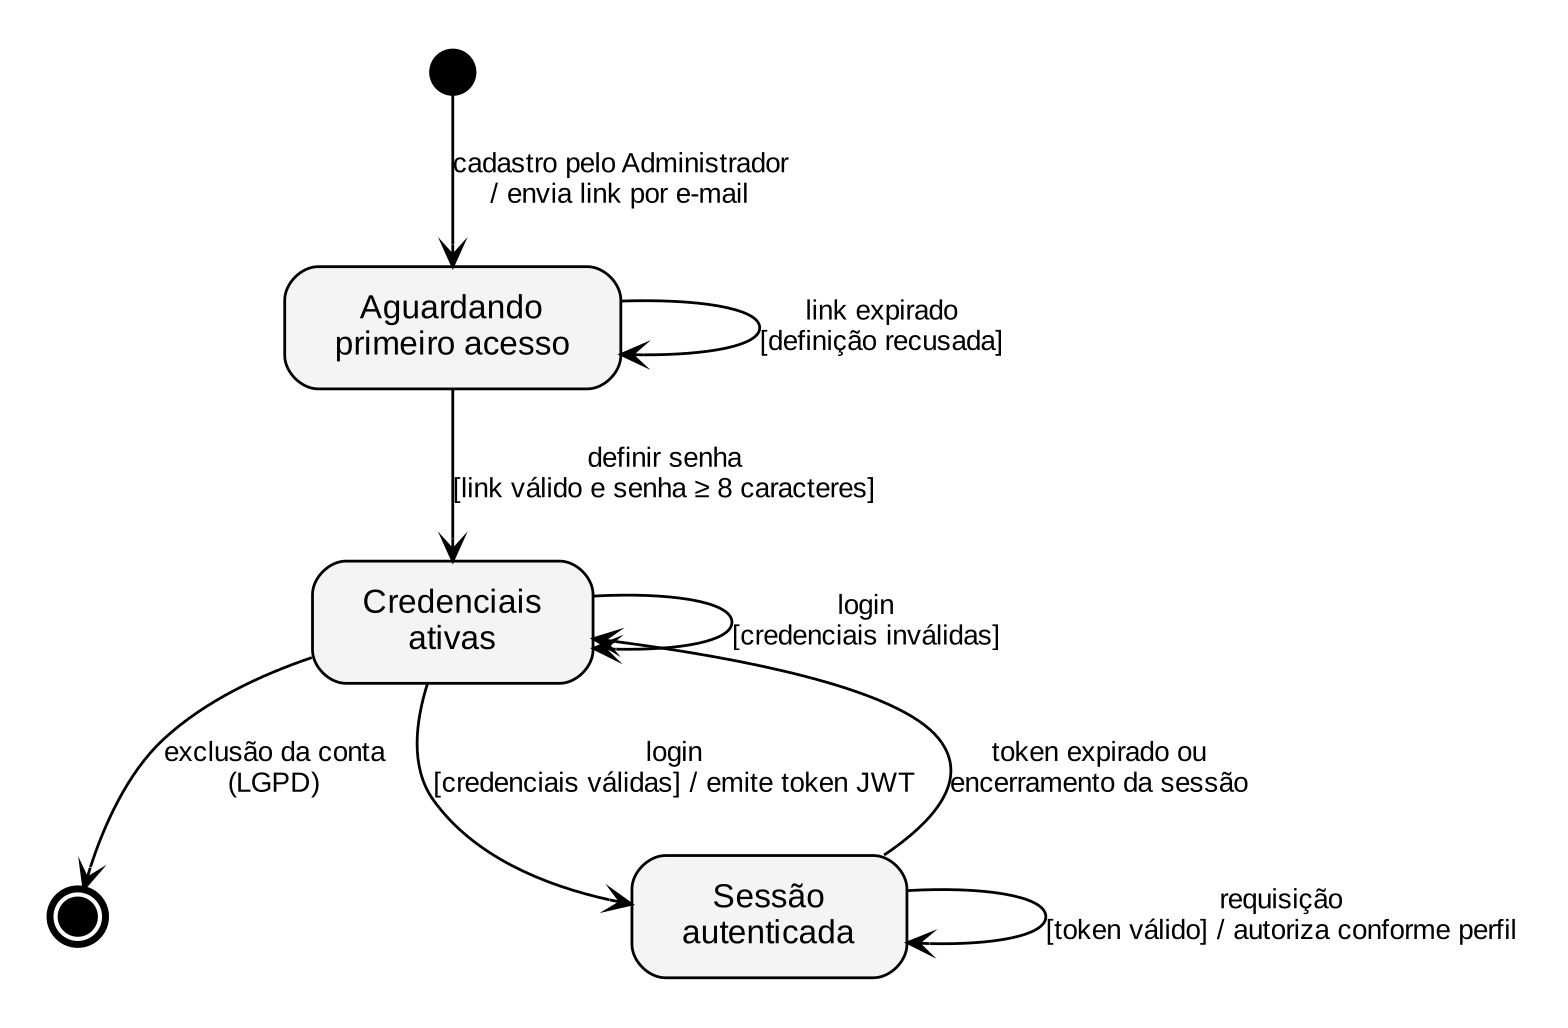
\includegraphics[width=0.77\textwidth]{img/fig-cap4-estados-acesso.png}
    \legend{Fonte: Autoria própria (2026).}
\end{figure}

\begin{figure}[H]
    \centering
    \caption{Diagrama de estados de uma trilha na jornada do aluno.}
    \label{fig_estados_trilha}
    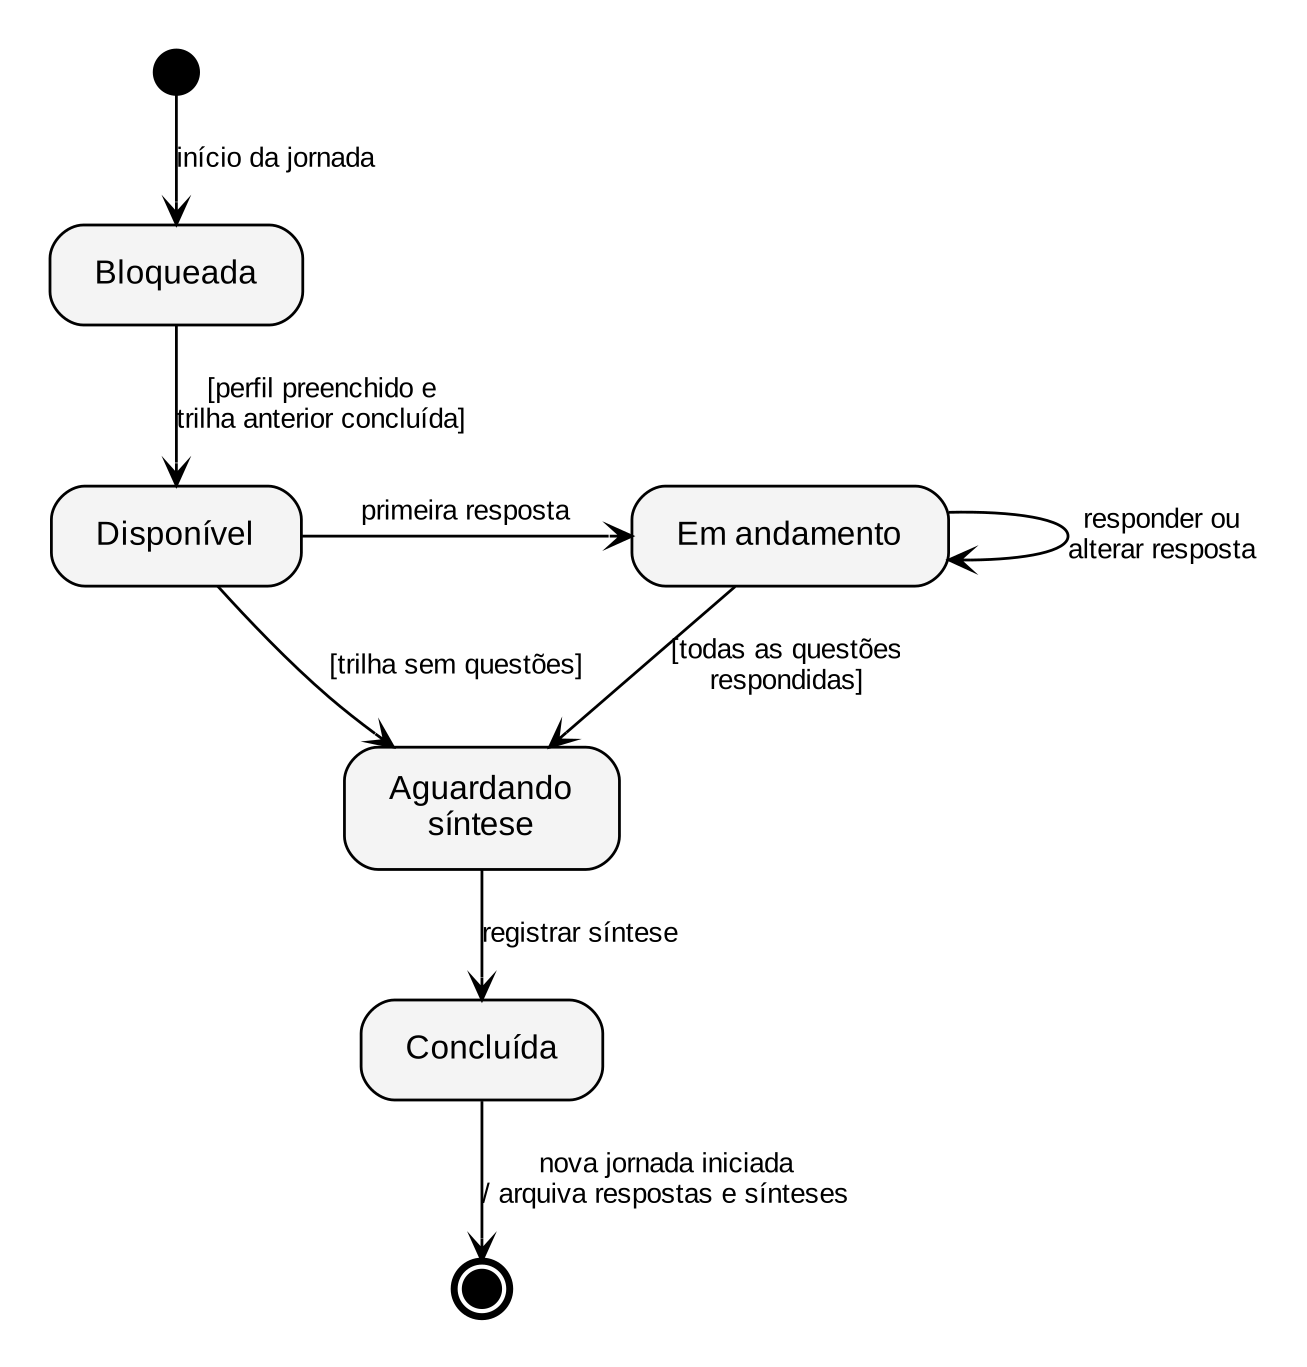
\includegraphics[width=0.66\textwidth]{img/fig-cap4-estados-trilha.png}
    \legend{Fonte: Autoria própria (2026).}
\end{figure}

\subsection{Proteção de dados}

Complementarmente, o sistema adota as seguintes medidas de proteção de dados:

\begin{itemize}
  \item \textbf{sigilo no painel gerencial}: o painel do profissional de orientação exibe apenas o progresso e a situação dos alunos, sem o conteúdo das respostas, conforme a regra de negócio RN-03;
  \item \textbf{eliminação de dados}: a exclusão de uma conta remove definitivamente os dados a ela associados, como sínteses, histórico de jornadas e \textit{feedbacks};
  \item \textbf{proteção de credenciais}: senhas armazenadas apenas na forma de \textit{hash} e \textit{tokens} de definição de senha com prazo de validade;
  \item \textbf{restrição de origens}: a API aceita requisições de navegador apenas das origens configuradas para a aplicação \textit{web} (CORS);
  \item \textbf{credenciais de serviços externos}: a autorização de acesso ao Google Agenda é concedida pelo próprio profissional de orientação e mantida apenas na memória da aplicação \textit{web}, sem armazenamento no servidor; as credenciais do servidor de e-mail são lidas de variáveis de ambiente.
\end{itemize}
